
\chapter{TikZ}
\label{cha:tikz}


\usetikzlibrary{arrows,snakes,backgrounds}

\section{Basics}
\label{sec:basics}



\subsection{Setting up the endironment}
\label{sec:sett-up-endir}

\begin{lstlisting}
\documentclass{article} % say
\usepackage{tikz}
\begin{document}
We are working on
\begin{tikzpicture}
  \draw (-1.5,0) -- (1.5,0);
  \draw (0,-1.5) -- (0,1.5);
\end{tikzpicture}.
\end{document}
\end{lstlisting}



We are working on
\begin{tikzpicture}
  \draw (-1.5,0) -- (1.5,0);
  \draw (0,-1.5) -- (0,1.5);
\end{tikzpicture}.



\begin{lstlisting}
\tikz \draw (-1.5,0) -- (1.5,0) -- (0,-1.5) -- (0,1.5);
\end{lstlisting}

\tikz \draw (-1.5,0) -- (1.5,0) -- (0,-1.5) -- (0,1.5);

\keyword{\textbackslash{}tikz} either takes one argument (starting with an opening braces) or collects everything up to the next semicolon and puts it inside a \keyword{tikzpicture} endironment.




\subsection{Straight path}
\label{sec:straight-path}

\begin{lstlisting}
\draw (0,0) -- (1.5,0);
\end{lstlisting}

\begin{tikzpicture}
  \draw (0,0) -- (1.5,0);
\end{tikzpicture}

The coordinates are used to locate the positions and \keyword{--} is used for drawing.

\subsection{Curved path}
\label{sec:curved-path}

\begin{lstlisting}
 \filldraw [gray] (0,0) circle (2pt)
                   (1,1) circle (2pt)
                   (2,1) circle (2pt)
                   (2,0) circle (2pt);
  \draw (0,0) .. controls (1,1) and (2,1) .. (2,0);
\end{lstlisting}


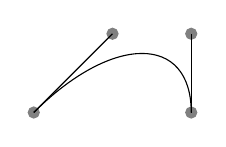
\begin{tikzpicture}
  \filldraw [gray] (0,0) circle (2pt)
  (1,1) circle (2pt)
  (2,1) circle (2pt)
  (2,0) circle (2pt);
  \draw (0,0) .. controls (1,1) and (2,1) .. (2,0);
  \draw (0,0) -- (1,1);
  \draw (2,1) -- (2,0);
\end{tikzpicture}

You can leave out the \keyword{and} (second control point), which causes the first one to be used twice.



\subsection{Circle path}
\label{sec:circle-path}

\begin{lstlisting}
\draw (0,0) circle (10pt);
\end{lstlisting}


\begin{tikzpicture}
  \draw (0,0) circle (10pt);
\end{tikzpicture}



\begin{lstlisting}
\draw (0,0) ellipse (20pt and 10pt);
\end{lstlisting}

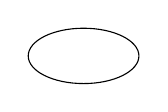
\begin{tikzpicture}
  \draw (0,0) ellipse (20pt and 10pt);
\end{tikzpicture}

\subsection{Rectangle path}
\label{sec:rectangle-path}

\begin{lstlisting}
\filldraw [gray] (0,0) circle (2pt);
\filldraw [gray] (0.5,0.5) circle (2pt);
  \draw (0,0) rectangle (0.5,0.5);
\end{lstlisting}


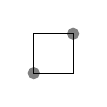
\begin{tikzpicture}
  \filldraw [gray] (0,0) circle (2pt);
  \filldraw [gray] (0.5,0.5) circle (2pt);
  \draw (0,0) rectangle (0.5,0.5);
\end{tikzpicture}

\subsection{Grid path}
\label{sec:grid-path}

\begin{lstlisting}
  \filldraw [gray] (-1.4,-1.4) circle (2pt);
  \filldraw [gray] (1.4,1.4) circle (2pt);

  \draw[step=.5cm,gray,very thin] (-1.4,-1.4) grid (1.4,1.4);
\end{lstlisting}


\begin{tikzpicture}
  \filldraw [gray] (-1.4,-1.4) circle (2pt);
  \filldraw [gray] (1.4,1.4) circle (2pt);

  \draw[step=.5cm,gray,very thin] (-1.4,-1.4) grid (1.4,1.4);
\end{tikzpicture}


\subsection{Arc path}
\label{sec:arc-path}

\begin{lstlisting}
  \filldraw [gray] (0,0) circle (2pt);
  \draw (0mm,0mm) arc (0:30:3cm);
  % (center) arc (angle1:angle2:radius)
  % an arc from angle1 to angle2 on a circle of radius

\end{lstlisting}


\begin{tikzpicture}
  \filldraw [gray] (0,0) circle (2pt);

  \draw (0mm,0mm) arc (0:30:3cm);
  % (center) arc (angle1:angle2:radius)
  % an arc from angle1 to angle2 on a circle of radius
\end{tikzpicture}



\subsection{Clipping a path}
\label{sec:clipping-path}
\begin{lstlisting}
  \draw[step=.5cm,gray,very thin] (-1.4,-1.4) grid (1.4,1.4);
  \draw (-1.5,0) -- (1.5,0);
  \draw (0,-1.5) -- (0,1.5);
  \draw (0,0) circle (1cm);
  \draw (3mm,0mm) arc (0:30:3mm);  

\end{lstlisting}

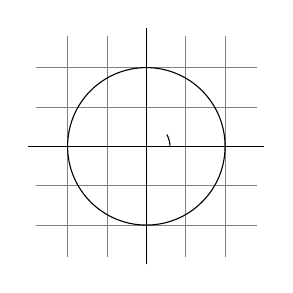
\begin{tikzpicture}
  \draw[step=.5cm,gray,very thin] (-1.4,-1.4) grid (1.4,1.4);
  \draw (-1.5,0) -- (1.5,0);
  \draw (0,-1.5) -- (0,1.5);
  \draw (0,0) circle (1cm);
  \draw (3mm,0mm) arc (0:30:3mm);  
\end{tikzpicture}

\begin{lstlisting}
  \clip (-0.1,-0.2) rectangle (1.1,0.75);
  \draw[step=.5cm,gray,very thin] (-1.4,-1.4) grid (1.4,1.4);
  \draw (-1.5,0) -- (1.5,0);
  \draw (0,-1.5) -- (0,1.5);
  \draw (0,0) circle (1cm);
  \draw (3mm,0mm) arc (0:30:3mm);  

\end{lstlisting}

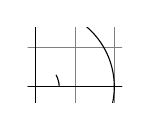
\begin{tikzpicture}
  \clip (-0.1,-0.2) rectangle (1.1,0.75);
  \draw[step=.5cm,gray,very thin] (-1.4,-1.4) grid (1.4,1.4);
  \draw (-1.5,0) -- (1.5,0);
  \draw (0,-1.5) -- (0,1.5);
  \draw (0,0) circle (1cm);
  \draw (3mm,0mm) arc (0:30:3mm);  
\end{tikzpicture}

In reality, \keyword{\textbackslash{}draw} is just a shorthand for \keyword{\textbackslash{}path[draw]} and \keyword{\textbackslash{}clip} is a shorthand for \keyword{\textbackslash{}path[clip]} and you could also say \keyword{\textbackslash{}path[draw,clip]}.



\subsection{Filling}
\label{sec:filling}

\begin{lstlisting}
\fill[green!20!white] (0,0) -- (3cm,0cm) arc (0:30:3cm) -- cycle;
\end{lstlisting}


\begin{tikzpicture}
  \fill[green!20!white] (0,0) -- (3cm,0cm) arc (0:30:3cm) -- cycle;
\end{tikzpicture}


The \keyword{--cycle} causes the current path to be closed.


You can also fill and draw a path at the same time using the \keyword{\textbackslash{}filldraw} command.


\subsection{Shading}
\label{sec:shading}

\keyword{\textbackslash{}shade} and \keyword{\textbackslash{}shadedraw} are used for shading and drawing at the same time.

\begin{lstlisting}
  \shade (0,0) rectangle (2,1);
  \shade[top color=yellow,bottom color=black] (3,0) rectangle +(2,1);
  \shade[left color=yellow,right color=black] (6,0) rectangle +(2,1); % relative coordinate
  \shadedraw[inner color=yellow,outer color=black,draw=yellow] (9,0) rectangle +(2,1);
  \shade[ball color=green] (12,.5) circle (.5cm);
\end{lstlisting}


\begin{tikzpicture}
  \shade (0,0) rectangle (2,1);
  \shade[top color=yellow,bottom color=black] (3,0) rectangle +(2,1);
  \shade[left color=yellow,right color=black] (6,0) rectangle +(2,1);
  \shadedraw[inner color=yellow,outer color=black,draw=yellow] (9,0) rectangle +(2,1);
  \shade[ball color=green] (12,.5) circle (.5cm);
\end{tikzpicture}

The default shading is a smooth transition from gray to white. To specify different colors, you can use options.



\subsection{Specifying coordinates}
\label{sec:spec-coord}

\begin{itemize}
\item If you leave out the unites, the default are set to cm and for angle to degree.
\item \keyword{+} means a relative coordinate from the previous specified position and \keyword{++} means a relative coordinate from the previous specified position, making this the new specified position.
\item You can use \keyword{intersection} to specify a coordinate.
\end{itemize}


\begin{lstlisting}
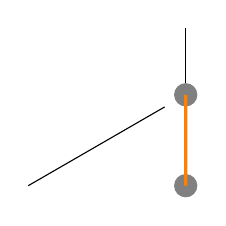
\begin{tikzpicture}[scale=2]
  \draw (1,0) -- (1,1);
  \draw (0,0) -- (30:1cm);
  \filldraw [gray] (1,0) circle (2pt);
  \filldraw [gray] (intersection of 1,0--1,1 and 0,0--30:1cm) circle (2pt);
  \draw[very thick,orange] (1,0) -- (intersection of 1,0--1,1 and 0,0--30:1cm);
\end{tikzpicture}

\end{lstlisting}

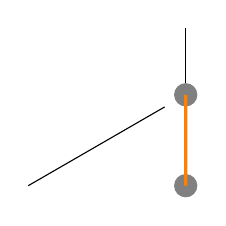
\begin{tikzpicture}[scale=2]
  \draw (1,0) -- (1,1);
  \draw (0,0) -- (30:1cm);
  \filldraw [gray] (1,0) circle (2pt);
  \filldraw [gray] (intersection of 1,0--1,1 and 0,0--30:1cm) circle (2pt);
  \draw[very thick,orange] (1,0) -- (intersection of 1,0--1,1 and 0,0--30:1cm);
\end{tikzpicture}


\subsection{Adding arrow tips}
\label{sec:adding-arrow}


\begin{lstlisting}
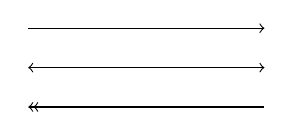
\begin{tikzpicture}
  \draw[->] (-1.5,0) -- (1.5,0);
  \draw[<->] (-1.5,-0.5) -- (1.5,-0.5);
  \draw[<<-] (-1.5,-1) -- (1.5,-1);
\end{tikzpicture}
\end{lstlisting}

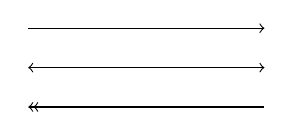
\begin{tikzpicture}
  \draw[->] (-1.5,0) -- (1.5,0);
  \draw[<->] (-1.5,-0.5) -- (1.5,-0.5);
  \draw[<<-] (-1.5,-1) -- (1.5,-1);
\end{tikzpicture}

\begin{lstlisting}
\begin{tikzpicture}[>=stealth]  % >= right arrow tip kind
  \draw[->] (-1.5,0) -- (1.5,0);
\end{tikzpicture}
\end{lstlisting}

\begin{tikzpicture}[>=stealth]  % >= right arrow tip kind
  \draw[->] (-1.5,0) -- (1.5,0);
\end{tikzpicture}



\subsection{Scoping}
\label{sec:scoping}

Scope can let you apply graphic options to a local group.

\begin{lstlisting}
\begin{tikzpicture}[ultra thick]
  \draw (0,0) -- (0,1);
  \begin{scope}[thin]
    \draw (1,0) -- (1,1);
    \draw (2,0) -- (2,1);
  \end{scope}
  \draw (3,0) -- (3,1);
\end{tikzpicture}
\end{lstlisting}

\begin{tikzpicture}[ultra thick]
  \draw (0,0) -- (0,1);
  \begin{scope}[thin]
    \draw (1,0) -- (1,1);
    \draw (2,0) -- (2,1);
  \end{scope}
  \draw (3,0) -- (3,1);
\end{tikzpicture}


\subsection{Transformations}
\label{sec:transformations}

When you specify a coordinate, TikZ applies certain transformations to the given coordinate in order to determine the finally position on the page.

\begin{lstlisting}

\begin{tikzpicture}[even odd rule,rounded corners=2pt,x=10pt,y=10pt]
  % x=10pt set the x unit to 10pt
  \filldraw (0,0)   rectangle (1,1)
  [xshift=5pt,yshift=5pt]   (0,0)   rectangle (1,1)
  [rotate=30]   (-1,-1) rectangle (2,2);

\end{tikzpicture}

\end{lstlisting}


\begin{tikzpicture}[even odd rule,rounded corners=2pt,x=10pt,y=10pt]
  % x=10pt set the x unit to 10pt
  \filldraw (0,0)   rectangle (1,1)
  [xshift=5pt,yshift=5pt]   (0,0)   rectangle (1,1)
  [rotate=30]   (-1,-1) rectangle (2,2);

\end{tikzpicture}

Options to do transformations:
\begin{itemize}
\item \keyword{xshift} and \keyword{yshift}
\item \lstinline|shift={(1,0)}| for shifting to a given point
\item \keyword{rotate} for rotating by a certain angle
\item \keyword{rotate around} for rotating around a given point
\item \keyword{scale} for scaling by a certain factor
\item \keyword{xscale} and \keyword{yscale} (\keyword{xscale=-1} is a flip)
\item \keyword{xslant} and \keyword{yslant} for slanting
\end{itemize}



\subsection{For-loops}
\label{sec:loops}
PGF introduces a command called \keyword{\textbackslash{}foreach}.
The general syntax is
\begin{lstlisting}
\foreach variable in {list of values} command
\end{lstlisting}

\begin{lstlisting}
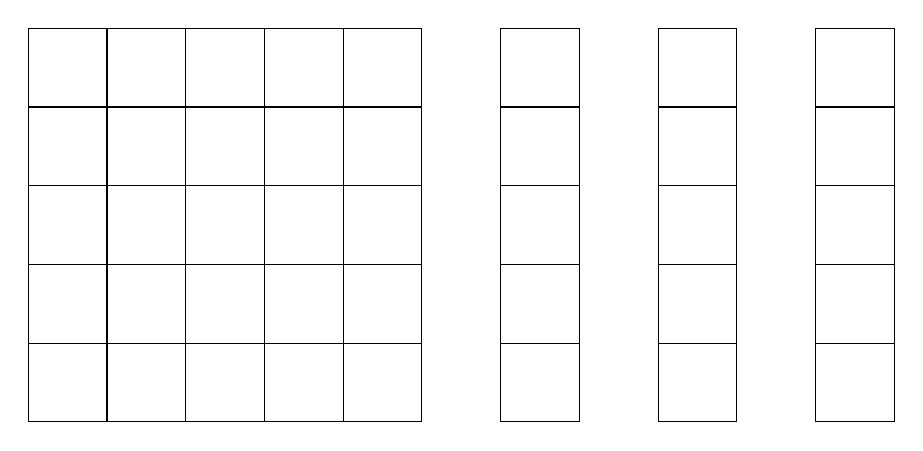
\begin{tikzpicture}
  \foreach \x in {1,2,...,5,7,9,...,12}
    \foreach \y in {1,...,5}
    {
      \draw (\x,\y) +(-.5,-.5) rectangle ++(.5,.5);
    }
\end{tikzpicture}

\end{lstlisting}

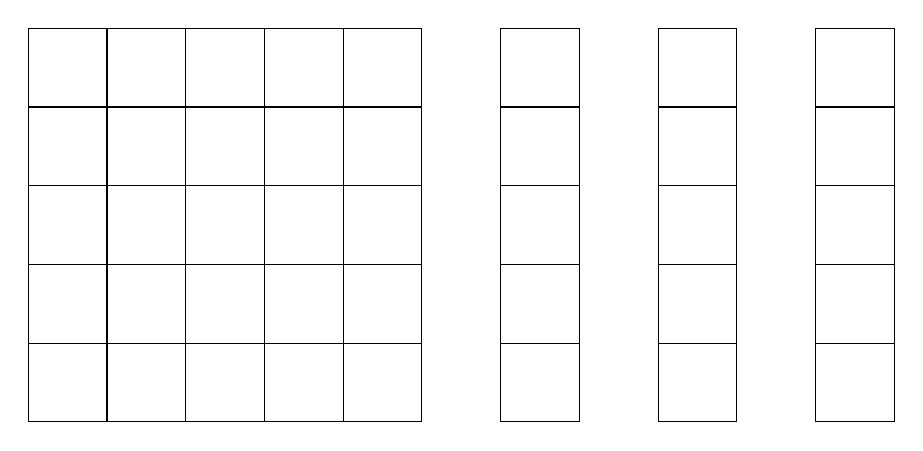
\begin{tikzpicture}
  \foreach \x in {1,2,...,5,7,9,...,12}
    \foreach \y in {1,...,5}
    {
      \draw (\x,\y) +(-.5,-.5) rectangle ++(.5,.5);
    }
\end{tikzpicture}

If you provide two numbers before the \keyword{...}, the \keyword{\textbackslash{}foreach} statement will use their difference for the stepping.




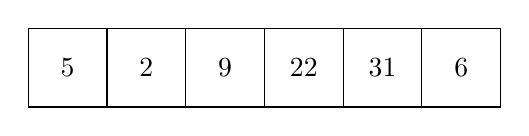
\begin{tikzpicture}
  \foreach \x\y in {0/5,1/2,2/9,3/22,4/31,5/6}
  {
    \node [rectangle,draw,minimum size=1cm] () at (\x ,0) {\y};
  }
\end{tikzpicture}

\begin{lstlisting}

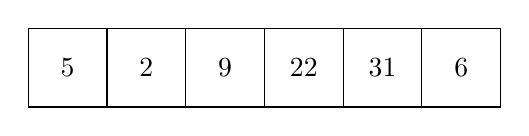
\begin{tikzpicture}
  \foreach \x\y in {0/5,1/2,2/9,3/22,4/31,5/6}
  {
    \node [rectangle,draw,minimum size=1cm] () at (\x ,0) {\y};
  }
\end{tikzpicture}
\end{lstlisting}
\subsection{Adding text}
\label{sec:adding-text}

\begin{lstlisting}
\begin{tikzpicture}
  \draw (0,0) -- node[above=1pt] {above=1pt} (3,0)
  (0,-1) -- node[anchor=north] {anchor=north} (3,-1);
  \draw (0,-3) .. controls (6,-2) and (9,-2) ..
  node[near start,sloped,above] {near start}
  node {midway}
  node[very near end,sloped,below] {very near end} (12,-3);
\end{tikzpicture}
\end{lstlisting}


\begin{tikzpicture}
  \draw (0,0) -- node[above=1pt] {above=1pt} (3,0)
  (0,-1) -- node[anchor=north] {anchor=north} (3,-1);
  \draw (0,-3) .. controls (6,-2) and (9,-2) ..
  node[near start,sloped,above] {near start}
  node {midway}
  node[very near end,sloped,below] {very near end} (12,-3);
\end{tikzpicture}

When TikZ is constructing a path and encounters the keyword \keyword{node} in the middle of a path, it reads a ``node specification''.
The keyword \keyword{node} is typically followed by some options and then some text between curly braces.
This text is put inside a normal TEX box.
All nodes are drawn only after the path has been completely drawn.
You can determine the direction to the position with the \keyword{anchor} option.
And there are simplified writing for the \keyword{anchor} option.
\keyword{below} does the same as \keyword{anchor=south east}.
You can also position labels on curves and, by adding the \keyword{sloped} option, have them rotated such that they match the line’s slope.

\subsection{Load library packages}
\label{sec:load-libr-pack}

\begin{lstlisting}
\usetikzlibrary{arrows,snakes,backgrounds}
\end{lstlisting}




\subsection{Set style}
\label{sec:set-style}

For some commonly used setting, you can set a short name for this setting to save typing and improve clarity.
\begin{lstlisting}
\tikzstyle{place}=[circle,draw=blue!50,fill=blue!20,thick, inner sep=0pt,minimum size=6mm]

\begin{tikzpicture}
  \node [place]  (waiting 1) at (0,2) {};
\end{tikzpicture}
\end{lstlisting}


\subsection{Set color}
\label{sec:set-color}

\begin{lstlisting}
\colorlet{anglecolor}{green!50!black}
\colorlet{sincolor}{red}

\filldraw[fill=green!20,draw=anglecolor] (0,0) -- (3mm,0pt) arc(0:30:3mm);
\end{lstlisting}


\subsection{Local definition}
\label{sec:local-definition}

\begin{lstlisting}
\def\costhirty{0.8660256}
\end{lstlisting}
\subsection{Node}
\label{sec:node}



A node have a \argument{position} and can have a \argument{shape} and \argument{name}.


The \funcword{\textbackslash{}node} command is an abbreviation for \funcword{\textbackslash{}path node}.

\begin{lstlisting}
% shape (circle), style (blue!50,fill=blue!20,thick), size (inner sep=0pt,minimum size=6mm)
\tikzstyle{place}=[circle,draw=blue!50,fill=blue!20,thick,
                   inner sep=0pt,minimum size=6mm]
\tikzstyle{transition}=[rectangle,draw=black!50,fill=black!20,thick,
                        inner sep=0pt,minimum size=4mm]
\begin{tikzpicture}
  % option   name   coordinate  text
  \node[place]      (waiting 1)      at ( 0,2) {};
  \node[place]      (critical 1)     at ( 0,1) {};
  \node[place]      (semaphore)      at ( 0,0) {};
  \node[transition] (leave critical) at ( 1,1) {};
  \node[transition] (enter critical) at (-1,1) {};
\end{tikzpicture}
\end{lstlisting}



% shape (circle), style (blue!50,fill=blue!20,thick), size (inner sep=0pt,minimum size=6mm)
\tikzstyle{place}=[circle,draw=blue!50,fill=blue!20,thick,
                   inner sep=0pt,minimum size=6mm]
\tikzstyle{transition}=[rectangle,draw=black!50,fill=black!20,thick,
                        inner sep=0pt,minimum size=4mm]
\begin{tikzpicture}
  % option   name   coordinate  text
  \node[place]      (waiting 1)      at ( 0,2) {};
  \node[place]      (critical 1)     at ( 0,1) {};
  \node[place]      (semaphore)      at ( 0,0) {};
  \node[transition] (leave critical) at ( 1,1) {};
  \node[transition] (enter critical) at (-1,1) {};
\end{tikzpicture}





We can use relative coordinates and add label to a node.
\begin{lstlisting}
\begin{tikzpicture}
  \tikzstyle{every label}=[red]
  \node[place]   (waiting)      {};                      
  \node[place]   (critical)     [below of=waiting]  {};  
  \node[place]   (semaphore)    [below of=critical,      
                                label=above:$s\le3$] {};   

  \node[transition] (leave critical) [right of=critical] {};
  \node[transition] (enter critical) [left of=critical]  {};
\end{tikzpicture}
\end{lstlisting}


\begin{tikzpicture}
  \tikzstyle{every label}=[red]
  \node[place]   (waiting)      {};                      
  \node[place]   (critical)     [below of=waiting]  {};  
  \node[place]   (semaphore)    [below of=critical,      
                                label=above:$s\le3$] {};   

  \node[transition] (leave critical) [right of=critical] {};
  \node[transition] (enter critical) [left of=critical]  {};
\end{tikzpicture}


We can use \keyword{edge} to draw connection lines.
\begin{lstlisting}
\tikzstyle{pre}=[<-,shorten <=1pt,>=stealth,semithick]
\tikzstyle{post}=[->,shorten >=1pt,>=stealth,semithick]
\begin{tikzpicture}[bend angle=45]
  \node[place]    (waiting)                            {};
  \node[place]    (critical)       [below of=waiting]  {};
  \node[place]    (semaphore)      [below of=critical] {};

  \node[transition] (leave critical) [right of=critical] {}
  edge [pre]                                 (critical)
  edge [post,bend right] node[auto,swap] {2} (waiting)
  edge [pre, bend left]                      (semaphore);
  \node[transition] (enter critical) [left of=critical]  {}
  edge [post]                              (critical) 
  edge [pre, bend left]                    (waiting)
  edge [post,bend right]                   (semaphore);
\end{tikzpicture}
\end{lstlisting}

\tikzstyle{pre}=[<-,shorten <=1pt,>=stealth,semithick]
\tikzstyle{post}=[->,shorten >=1pt,>=stealth,semithick]
\begin{tikzpicture}[bend angle=45]
  \node[place]    (waiting)                            {};
  \node[place]    (critical)       [below of=waiting]  {};
  \node[place]    (semaphore)      [below of=critical] {};

  \node[transition] (leave critical) [right of=critical] {}
  edge [pre]                                 (critical)
  edge [post,bend right] node[auto,swap] {2} (waiting)
  edge [pre, bend left]                      (semaphore);
  \node[transition] (enter critical) [left of=critical]  {}
  edge [post]                              (critical) 
  edge [pre, bend left]                    (waiting)
  edge [post,bend right]                   (semaphore);
\end{tikzpicture}



\subsection{Snake line}
\label{sec:snake-line}
\usetikzlibrary{snakes}
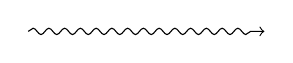
\begin{tikzpicture}
  \draw [->,snake=snake,
         segment amplitude=.4mm,
         segment length=2mm,
         line after snake=1mm] (0,0) -- (3,0);
\end{tikzpicture}


\begin{lstlisting}

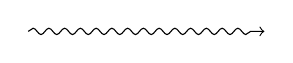
\begin{tikzpicture}
  \draw [->,snake=snake,
         segment amplitude=.4mm,
         segment length=2mm,
         line after snake=1mm] (0,0) -- (3,0);
\end{tikzpicture}
\end{lstlisting}
\section{Examples}
\label{sec:examples}

\subsection{A picture for Karl’s students}
\label{sec:pict-karls-stud}

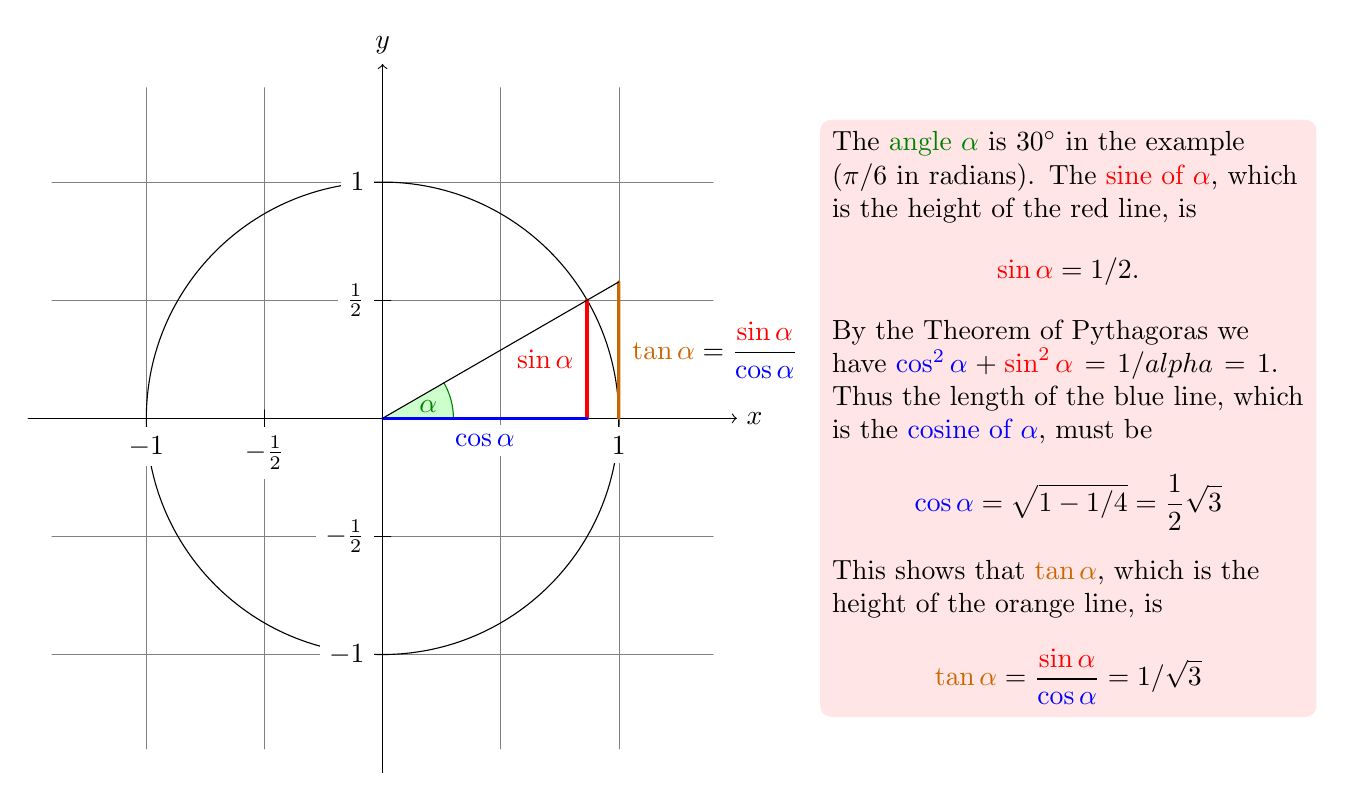
\begin{tikzpicture}[scale=3,cap=round]
  % Local definitions
  \def\costhirty{0.8660256}
  % Colors
  \colorlet{anglecolor}{green!50!black}
  \colorlet{sincolor}{red}
  \colorlet{tancolor}{orange!80!black}
  \colorlet{coscolor}{blue}
  % Styles
  \tikzstyle{axes}=[]
  \tikzstyle{important line}=[very thick]
  \tikzstyle{information text}=[rounded corners,fill=red!10,inner sep=1ex]
  % The graphic
  \draw[style=help lines,step=0.5cm] (-1.4,-1.4) grid (1.4,1.4);
  \draw (0,0) circle (1cm);
  \begin{scope}[style=axes]
    \draw[->] (-1.5,0) -- (1.5,0) node[right] {$x$} coordinate(x axis);
    \draw[->] (0,-1.5) -- (0,1.5) node[above] {$y$} coordinate(y axis);
    \foreach \x/\xtext in {-1, -.5/-\frac{1}{2}, 1}
    \draw[xshift=\x cm] (0pt,1pt) -- (0pt,-1pt) node[below,fill=white] {$\xtext$};
    \foreach \y/\ytext in {-1, -.5/-\frac{1}{2}, .5/\frac{1}{2}, 1}
    \draw[yshift=\y cm] (1pt,0pt) -- (-1pt,0pt) node[left,fill=white] {$\ytext$};
  \end{scope}
  \filldraw[fill=green!20,draw=anglecolor] (0,0) -- (3mm,0pt) arc(0:30:3mm);
  \draw (15:2mm) node[anglecolor] {$\alpha$};
  \draw[style=important line,sincolor]
  (30:1cm) -- node[left=1pt,fill=white] {$\sin \alpha$} (30:1cm |- x axis);
  \draw[style=important line,coscolor]
  (30:1cm |- x axis) -- node[below=2pt,fill=white] {$\cos \alpha$} (0,0);
  \draw[style=important line,tancolor] (1,0) -- node[right=1pt,fill=white] {
    $\displaystyle \tan \alpha \color{black}=
    \frac{{\color{sincolor}\sin \alpha}}{\color{coscolor}\cos \alpha}$}
  (intersection of 0,0--30:1cm and 1,0--1,1) coordinate (t);
  \draw (0,0) -- (t);
  \draw[xshift=1.85cm]
  node[right,text width=6cm,style=information text]
  {
    The {\color{anglecolor} angle $\alpha$} is $30^\circ$ in the
      example ($\pi/6$ in radians). The {\color{sincolor}sine of
        $\alpha$}, which is the height of the red line, is
      \[
      {\color{sincolor} \sin \alpha} = 1/2.
      \]

      By the Theorem of Pythagoras we have ${\color{coscolor}\cos ^2 \alpha}+{\color{sincolor} \sin^{2} \alpha} = 1/alpha=1$.
      Thus the length of the blue line, which is the {\color{coscolor} cosine of $\alpha$}, must be
    $$
    {\color{coscolor}\cos \alpha}=\sqrt{1-1 / 4}=\frac{1}{2} \sqrt{3}
    $$
    This shows that {\color{tancolor}$\tan \alpha$}, which is the height of the orange line, is
    $$
    {\color{tancolor}\tan \alpha}=\frac{\color{sincolor}\sin \alpha}{\color{coscolor}\cos \alpha}=1 / \sqrt{3}
    $$
  };
\end{tikzpicture}

\begin{lstlisting}
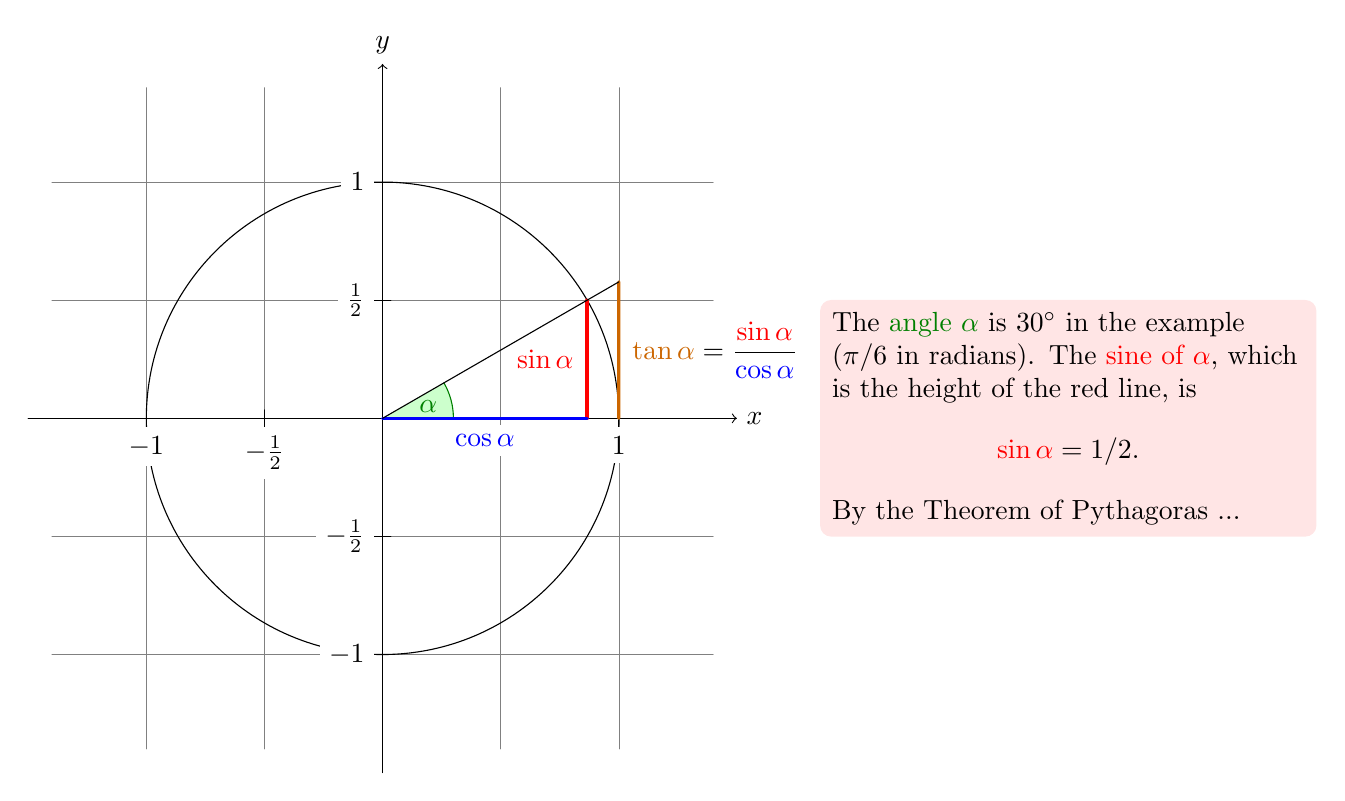
\begin{tikzpicture}[scale=3,cap=round]
% Local definitions
  \def\costhirty{0.8660256}
% Colors
  \colorlet{anglecolor}{green!50!black}
  \colorlet{sincolor}{red}
  \colorlet{tancolor}{orange!80!black}
  \colorlet{coscolor}{blue}
% Styles
  \tikzstyle{axes}=[]
  \tikzstyle{important line}=[very thick]
  \tikzstyle{information text}=[rounded corners,fill=red!10,inner sep=1ex]
% The graphic
  \draw[style=help lines,step=0.5cm] (-1.4,-1.4) grid (1.4,1.4);
  \draw (0,0) circle (1cm);
  \begin{scope}[style=axes]
    \draw[->] (-1.5,0) -- (1.5,0) node[right] {$x$} coordinate(x axis);
    \draw[->] (0,-1.5) -- (0,1.5) node[above] {$y$} coordinate(y axis);
    \foreach \x/\xtext in {-1, -.5/-\frac{1}{2}, 1}
      \draw[xshift=\x cm] (0pt,1pt) -- (0pt,-1pt) node[below,fill=white] {$\xtext$};
    \foreach \y/\ytext in {-1, -.5/-\frac{1}{2}, .5/\frac{1}{2}, 1}
      \draw[yshift=\y cm] (1pt,0pt) -- (-1pt,0pt) node[left,fill=white] {$\ytext$};
\end{scope}
  \filldraw[fill=green!20,draw=anglecolor] (0,0) -- (3mm,0pt) arc(0:30:3mm);
  \draw (15:2mm) node[anglecolor] {$\alpha$};
  \draw[style=important line,sincolor]
    (30:1cm) -- node[left=1pt,fill=white] {$\sin \alpha$} (30:1cm |- x axis);
  \draw[style=important line,coscolor]
    (30:1cm |- x axis) -- node[below=2pt,fill=white] {$\cos \alpha$} (0,0);
  \draw[style=important line,tancolor] (1,0) -- node[right=1pt,fill=white] {
    $\displaystyle \tan \alpha \color{black}=
    \frac{{\color{sincolor}\sin \alpha}}{\color{coscolor}\cos \alpha}$}
    (intersection of 0,0--30:1cm and 1,0--1,1) coordinate (t);
  \draw (0,0) -- (t);
  \draw[xshift=1.85cm]
    node[right,text width=6cm,style=information text]
    {
      The {\color{anglecolor} angle $\alpha$} is $30^\circ$ in the
      example ($\pi/6$ in radians). The {\color{sincolor}sine of
        $\alpha$}, which is the height of the red line, is
      \[
      {\color{sincolor} \sin \alpha} = 1/2.
      \]
      By the Theorem of Pythagoras ...
    };
\end{tikzpicture}
\end{lstlisting}



\subsection{A Petri-Net for Hagen}
\label{sec:petri-net-hagen}

\usetikzlibrary{arrows,snakes,backgrounds}

\tikzstyle{place}=[circle,draw=blue!50,fill=blue!20,thick,inner sep=0pt,minimum size=6mm]
\tikzstyle{transition}=[rectangle,draw=black!50,fill=black!20,thick,inner sep=0pt,minimum size=4mm]

\tikzstyle{pre}=[<-,shorten <=1pt,>=stealth,semithick]
\tikzstyle{post}=[->,shorten >=1pt,>=stealth,semithick]

\tikzstyle{every place}=[minimum size=6cm,thick,draw=blue!75,fill=blue!20]
\tikzstyle{every transition}=[thick,draw=black!75,fill=black!20]
\tikzstyle{red place}=[place,draw=red!75,fill=red!20]
\tikzstyle{every label}=[red]


\begin{tikzpicture}[node distance=1.3cm,>=stealth,bend angle=45,auto]
  \node [place] (w1)  {};
  \node [place] (c1) [below of=w1] {};
  \node [place] (s) [below of=c1,label=above:\(s\le 3\)] {};
  \node [place] (c2) [below of=s] {};
  \node [place] (w2) [below of=c2] {};

  \node [transition] (e1) [left of=c1] {}
  edge [pre,bend left] (w1)
  edge [post,bend right] (s)
  edge [post] (c1);
  \node [transition] (e2) [left of=c2] {}
  edge [pre, bend right] (w2)
  edge [pre, bend left] (s)
  edge [post] (c2);
  \node [transition] (l1) [right of=c1] {}
  edge [pre] (c1)
  edge [pre,bend left] (s)
  edge [post,bend right] node [swap] {2} (w1);
  \node [transition] (l2) [right of=c2] {}
  edge [pre] (c2)
  edge [pre,bend right] (s)
  edge [post,bend left] node {2} (w2);

  \begin{scope}[xshift=6cm]
    \node [place] (w1') {};
    \node [place] (c1') [below of=w1'] {};
    \node [red place] (s1') [below of=c1',xshift=-0.5cm] [label=left:\(s\)] {};
    \node [red place] (s2') [below of=c1',xshift=0.5cm] [label=right:\(\bar s\)] {};
    \node [place] (c2') [below of=s1',xshift=.5cm] {};
    \node [place] (w2') [below of=c2'] {};

    \node [transition] (e1') [left of=c1'] {}
    edge [pre,bend left] (w1')
    edge [post] (s1')
    edge [pre] (s2')
    edge [post] (c1');
    \node [transition] (e2') [left of=c2'] {}
    edge [pre,bend right] (w2')
    edge [post] (s1')
    edge [pre] (s2')
    edge [post] (c2');
    \node [transition] (l1') [right of=c1'] {}
    edge [pre] (c1')
    edge [pre] (s1')
    edge [post] (s2')
    edge [post,bend right] node [swap]  {2} (w1');
    \node [transition] (l2') [right of=c2'] {}
    edge [pre] (c2')
    edge [pre] (s1')
    edge [post] (s2')
    edge [post,bend left] node {2} (w2');
  \end{scope}

  \draw [-to,thick,snake=snake,segment amplitude=.4mm,segment length=2mm,line after snake=1mm]
    ([xshift=5mm]s -| l1) -- ([xshift=-5mm]s1' -| e1')
    node [above=1mm,midway,text width=3cm,text centered]
      {replacement of the \textcolor{red}{capacity} by \textcolor{red}{two places}};
  \begin{pgfonlayer}{background}
    \filldraw [line width=4mm,join=round,black!10]
      (w1.north  -| l1.east)  rectangle (w2.south  -| e1.west)
      (w1'.north -| l1'.east) rectangle (w2'.south -| e1'.west);
  \end{pgfonlayer}
\end{tikzpicture}


\begin{lstlisting}
\usetikzlibrary{arrows,snakes,backgrounds}

\tikzstyle{place}=[circle,draw=blue!50,fill=blue!20,thick,inner sep=0pt,minimum size=6mm]
\tikzstyle{transition}=[rectangle,draw=black!50,fill=black!20,thick,inner sep=0pt,minimum size=4mm]

\tikzstyle{pre}=[<-,shorten <=1pt,>=stealth,semithick]
\tikzstyle{post}=[->,shorten >=1pt,>=stealth,semithick]

\tikzstyle{every place}=[minimum size=6cm,thick,draw=blue!75,fill=blue!20]
\tikzstyle{every transition}=[thick,draw=black!75,fill=black!20]
\tikzstyle{red place}=[place,draw=red!75,fill=red!20]
\tikzstyle{every label}=[red]


\begin{tikzpicture}[node distance=1.3cm,>=stealth,bend angle=45,auto]
  \node [place] (w1)  {};
  \node [place] (c1) [below of=w1] {};
  \node [place] (s) [below of=c1,label=above:\(s\le 3\)] {};
  \node [place] (c2) [below of=s] {};
  \node [place] (w2) [below of=c2] {};

  \node [transition] (e1) [left of=c1] {}
  edge [pre,bend left] (w1)
  edge [post,bend right] (s)
  edge [post] (c1);
  \node [transition] (e2) [left of=c2] {}
  edge [pre, bend right] (w2)
  edge [pre, bend left] (s)
  edge [post] (c2);
  \node [transition] (l1) [right of=c1] {}
  edge [pre] (c1)
  edge [pre,bend left] (s)
  edge [post,bend right] node [swap] {2} (w1);
  \node [transition] (l2) [right of=c2] {}
  edge [pre] (c2)
  edge [pre,bend right] (s)
  edge [post,bend left] node {2} (w2);

  \begin{scope}[xshift=6cm]
    \node [place] (w1') {};
    \node [place] (c1') [below of=w1'] {};
    \node [red place] (s1') [below of=c1',xshift=-0.5cm] [label=left:\(s\)] {};
    \node [red place] (s2') [below of=c1',xshift=0.5cm] [label=right:\(\bar s\)] {};
    \node [place] (c2') [below of=s1',xshift=.5cm] {};
    \node [place] (w2') [below of=c2'] {};

    \node [transition] (e1') [left of=c1'] {}
    edge [pre,bend left] (w1')
    edge [post] (s1')
    edge [pre] (s2')
    edge [post] (c1');
    \node [transition] (e2') [left of=c2'] {}
    edge [pre,bend right] (w2')
    edge [post] (s1')
    edge [pre] (s2')
    edge [post] (c2');
    \node [transition] (l1') [right of=c1'] {}
    edge [pre] (c1')
    edge [pre] (s1')
    edge [post] (s2')
    edge [post,bend right] node [swap]  {2} (w1');
    \node [transition] (l2') [right of=c2'] {}
    edge [pre] (c2')
    edge [pre] (s1')
    edge [post] (s2')
    edge [post,bend left] node {2} (w2');
  \end{scope}

  \draw [-to,thick,snake=snake,segment amplitude=.4mm,segment length=2mm,line after snake=1mm]
    ([xshift=5mm]s -| l1) -- ([xshift=-5mm]s1' -| e1')
    node [above=1mm,midway,text width=3cm,text centered]
      {replacement of the \textcolor{red}{capacity} by \textcolor{red}{two places}};
  \begin{pgfonlayer}{background}
    \filldraw [line width=4mm,join=round,black!10]
      (w1.north  -| l1.east)  rectangle (w2.south  -| e1.west)
      (w1'.north -| l1'.east) rectangle (w2'.south -| e1'.west);
  \end{pgfonlayer}
\end{tikzpicture}

\end{lstlisting}
%%% Local Variables:
%%% mode: latex
%%% TeX-master: "latex"
%%% End:
